\documentclass[journal]{IEEEtran}

\usepackage{amsmath,amssymb}
\usepackage{graphicx}
\usepackage{booktabs}
\usepackage{algorithmic}
\usepackage{algorithm}
\usepackage{url}
\usepackage{tikz}
\usetikzlibrary{shapes.geometric,arrows.meta,positioning}
\graphicspath{{../paper/figures/}}

\begin{document}

\title{Physics-Constrained Repair of Quantum Circuits:\\
An Audited Benchmark, a Leakage-Free Protocol,\\
and Controlled Ablations}

\author{Alok~Pandey%
\thanks{The author is with the Indian Institute of Technology Patna, India.}%
\thanks{Code, data, per-attempt results and the analysis scripts required to
reproduce every number in this paper are available at
\protect\url{https://github.com/alok-108/physics-constrained-quantum-repair}.}}

\markboth{Manuscript draft}{Pandey: Physics-Constrained Repair of Quantum Circuits}

\maketitle

\begin{abstract}
Success rates reported for automated quantum-circuit repair are only meaningful
if the repair procedure cannot read the reference it is scored against and the
benchmark itself is valid. We audit the first release of this physics-constrained
repair framework and its benchmark and find both conditions violated: the reference
circuit was returned as the repair, baseline outcomes were hard-coded, 367 of
1000 reference circuits failed the validator's own connectivity check, and the
semantic check was blind to controlled-phase faults in the QFT. We specify a
protocol that fixes these defects (a query-counted behavioural oracle as the only
information channel, an exact-unitary and noise-floor acceptance predicate,
deterministic verdicts), release a corrected 1000-circuit benchmark whose
references are hardware-admissible and whose faults are observable by
construction, and evaluate a repair agent (analytic rotation-angle solving,
oracle-guided edit search, counterexample-guided feedback) in a $2\times2$
design that separates physical knowledge from feedback. At a matched attempt
budget of three, the full agent is accepted on $97.0\%$ of circuits (95\% CI
$[95.7,97.9]$) against $77.0\%$ without physical knowledge, $60.0\%$ for static
repair without an oracle, $29.7\%$ for the Qiskit transpiler alone and $5.0\%$ for
ZX-calculus simplification. The
physical-knowledge effect ($+20.0$ points, 200 discordant circuits, none
reversed) is confined to the physical fault class, where an arm without routing
cannot succeed; on logical faults the arms are indistinguishable. Diagnostic
feedback has no effect when the oracle is strong but raises Pass@3 from $88.1\%$
to $97.0\%$ ($+8.9$ points, $p<10^{-24}$) when the initial test suite is a single
state. No language model was executed; all results concern the deterministic
agent.
\end{abstract}

\begin{IEEEkeywords}
Quantum software engineering, automated program repair, circuit debugging,
hardware-aware compilation, benchmark validity, evaluation methodology.
\end{IEEEkeywords}

\section{Introduction}

A quantum program must satisfy two conditions that are easy to conflate: it must
compute what the specification demands, and it must be executable on the target
device~\cite{preskill2018nisq}. A repair that fixes a parser error can introduce
a wrong operand; a semantically correct abstract circuit can still violate
connectivity or exceed a coherence budget. Evaluating a repair system therefore
needs an acceptance predicate covering both, and a benchmark in which that
predicate can actually be satisfied by a correct repair.

Recent work studies language-model-assisted repair through direct patch
generation~\cite{guo2024chatgpt} and through agentic pipelines with bug
injection, detection, repair and simulation-based
validation~\cite{pham2026qbuglm}, alongside symbolic and learned circuit
transformation~\cite{duncan2020zx,kissinger2020pyzx,li2024quarl}. The common
evaluation pattern is to compare a candidate with a reference circuit and report
agreement as success. This is sound only if (i) the repair procedure could not
have consulted the reference, (ii) the reference is itself acceptable under the
predicate, and (iii) every injected fault is detectable by that predicate. In a
multi-component agent the reference tends to be reachable somewhere in the call
graph, and benchmarks generated by script are rarely checked against their own
validator.

We examined the first release of this repository's physics-constrained repair
framework and benchmark for exactly these properties and report what we found
(Section~\ref{sec:audit}). The results
it originally reported (Pass@1 $77.5\%$, Pass@3 $99.1\%$) cannot be used. This
paper makes the following contributions.

\begin{enumerate}
\item \textbf{An audit} of the original harness and benchmark, with a reusable
tool (\texttt{src/audit.py}) that checks reference admissibility and fault
observability on any dataset.
\item \textbf{A leakage-free protocol}: an explicit information boundary, a
query-counted behavioural oracle, a deterministic acceptance predicate with an
exact noise-floor criterion, and a held-out overfitting measurement.
\item \textbf{Benchmark v2}: 1000 circuits with hardware-admissible references and
verified-observable faults, labelled by fault mode so results can be read per
mode rather than only per class.
\item \textbf{A repair agent} using analytic rotation-angle solving,
meet-in-the-middle scoring of whole edit neighbourhoods, tabu diversification,
and counterexample-guided feedback.
\item \textbf{Controlled experiments}: a $2\times2$ factorial design
(physical knowledge $\times$ feedback) with a no-oracle lower bound and a
transformation baseline, a weak-oracle regime, and a query-budget sweep.
\end{enumerate}

We state limits up front. The benchmark consists of small edits of short
circuits whose inverse lies inside the agent's edit neighbourhood, so a high rate
on single-edit faults is expected and is not evidence of general repair ability;
the informative cells are the fault modes outside the neighbourhood and the
weak-oracle and low-budget regimes. Hardware is a device model, connectivity is
checked under the identity layout, and no language model was run.

\section{Related Work and Scope}

\textbf{Language-guided repair.} Guo \emph{et al.}~\cite{guo2024chatgpt} apply
ChatGPT to repair quantum programs. QBugLM~\cite{pham2026qbuglm} provides an
agentic benchmarking framework and reports that iterative feedback matters. Any
comparison with such a system must match retry budgets and run the authors'
release; we therefore report no arm named after an external system. Published
quantum repair methods with their own protocols include HornBro~\cite{tan2025hornbro}
and the unitary-operation approach of Li \emph{et al.}~\cite{li2024unitar}; they
differ from ours in task, language and oracle, so we do not claim a head-to-head
comparison with them.

\textbf{Benchmarks.} Bugs4Q~\cite{zhao2023bugs4q} remains the main collection of
real, executable quantum bugs with reproducing tests, but it is small and tied to
Qiskit, and its entries are sensitive to SDK versions; reproducibility drops
without version pinning~\cite{ohto2026reproducibility}. Our benchmark is
synthetic and therefore complementary: it trades realism for control over
admissibility and observability, and it makes no claim about real-fault
prevalence. Surveys of quantum testing identify the oracle problem as central
and stress methodological standards~\cite{ramalho2024roadmap}; measurement-based
oracles that use only computational-basis outputs can miss phase
faults~\cite{oldfield2024projective}, which is the failure we found in the
single-input check.

\textbf{Transformation baselines.} ZX-calculus simplification~\cite{duncan2020zx}
rewrites a circuit while preserving the computation it denotes, which makes PyZX
a meaningful transformation baseline but not a repair baseline: it cannot restore
a computation the faulty circuit does not implement. Quarl~\cite{li2024quarl}
learns a rewriting policy and meets the same boundary.

\textbf{Test-suite-guided repair.} In classical program repair the tool receives
a test suite, not the fixed program~\cite{legoues2012genprog}, and overfitting to
that suite is a known hazard~\cite{smith2015overfitting}. Counterexample-guided
inductive synthesis~\cite{solarlezama2006sketching} adds failing inputs to the
suite. Our oracle and feedback arms transplant both ideas to circuits.

\textbf{Parameter optimisation.} For a circuit with one free rotation angle, a
measured quantity is a low-degree trigonometric polynomial of that angle, so its
optimum can be located analytically from a few evaluations; this underlies
sequential minimal optimisation~\cite{nakanishi2020sequential} and structure
optimisation~\cite{ostaszewski2021structure} for variational circuits. We use the
same property to repair a wrong angle in three oracle queries.

\textbf{Execution models.} Hardware checks use the FakeSherbrooke backend model;
backend-derived noise models approximate device behaviour~\cite{ibmnoise}, so
passing them is distinct from fidelity on a live processor.

\section{Audit of the Original Benchmark}
\label{sec:audit}

We audited the original release against its own validator. Table~\ref{tab:audit}
summarises the findings; per-defect locations and fixes are in
\texttt{docs/BENCHMARK\_V2.md}.

\begin{table}[t]
\centering
\caption{Audit of the original (v1) harness and benchmark. Counts are over its
1000 circuits unless stated.}
\label{tab:audit}
\footnotesize
\setlength{\tabcolsep}{3pt}
\begin{tabular}{p{0.66\columnwidth}p{0.24\columnwidth}}
\toprule
Finding & Evidence \\
\midrule
Reference circuit returned as the repair (\texttt{ground\_truth\_hint}) & code \\
Baseline outcome hard-coded to failure for all physics-fault circuits & code \\
Baseline Pass@3 set equal to Pass@1 (one attempt vs.\ three) & code \\
Arm named ``QBugLM'' was the project's own repairer & code \\
Injected fault label passed to the diagnostician & code \\
Reference circuits failing the validator's connectivity check & 367 (250 QFT, 117 QAOA) \\
Structural/semantic faults that leave the unitary unchanged & 20 of 400 \\
Single-input semantic check blind to QFT phase and swap faults & fidelity $1.0000$ \\
No acceptance stage separating a redundant circuit from its reference & by construction \\
\bottomrule
\end{tabular}
\end{table}

The connectivity and blindness findings are not harness bugs but properties of the
benchmark and predicate, and they survive fixing the leakage. First, a candidate
can be semantically perfect and still be rejected, and any system lacking a
routing step cannot pass those circuits; the apparent value of ``physical
awareness'' then depends on circuit family rather than on the injected fault.
Second, a QFT acting on $\lvert 0\ldots0\rangle$ yields the uniform
superposition, so a circuit consisting only of the Hadamard layer and a circuit
with every controlled phase negated both have overlap $1.0000$ with the
reference (checked on real references); such faults are unobservable under a
single-input check.

\section{Evaluation Protocol}
\label{sec:protocol}

\subsection{Information boundary}

Let $\mathcal{I}_R$ be the information available to the repair procedure and
$\mathcal{I}_V$ that available to the acceptance predicate. A valid evaluation
requires
\begin{equation}
\label{eq:boundary}
C_{\mathrm{ref}} \in \mathcal{I}_V,\quad C_{\mathrm{ref}} \notin \mathcal{I}_R,\quad
\beta \notin \mathcal{I}_R,
\end{equation}
where $C_{\mathrm{ref}}$ is the reference and $\beta$ the injected fault class
and mode. If $C_{\mathrm{ref}}\in\mathcal{I}_R$ the trivial procedure that emits
it is accepted on every circuit; if $\beta\in\mathcal{I}_R$ localisation is
handed its answer. We enforce~\eqref{eq:boundary} in code: the benchmark's
annotation fields are stripped from the specification before any repair-side
component sees it, the \texttt{repair} interface has no reference argument, and
unit tests check both.

\subsection{Behavioural oracle}

The reference is wrapped in an oracle that exposes only a scalar agreement score
and a query counter. It privately holds three disjoint sets of input states:
a \emph{suite} guiding the search ($\lvert 0\ldots0\rangle$ plus
Haar-random product states), a \emph{pool} of candidate counterexamples, and a
\emph{held-out} set never used for search or feedback. The score of a candidate
$C$ is the mean agreement $\Omega(C)=\tfrac{1}{m}\sum_{j}\lvert\langle
\psi^{\mathrm{ref}}_j\mid\psi^{C}_j\rangle\rvert^2$ over the current suite.
Every scored edit, \texttt{score} call and counterexample request consumes one
query of a per-repair budget (default 8000). The oracle's search signal is
deliberately weaker than the acceptance predicate: the latter checks the full
unitary, which makes overfitting measurable as the gap between suite agreement
and exact process fidelity of the final candidate.

\subsection{Acceptance predicate}

Acceptance is a conjunction, evaluated from inexpensive to expensive stages and
identical for every system:
\begin{equation}
\mathcal{A}(C;R,B)=V_{\mathrm{syn}}\wedge V_{\mathrm{str}}\wedge V_{\mathrm{phys}}
\wedge V_{\mathrm{min}}\wedge V_{\mathrm{sem}}\wedge V_{\mathrm{noise}}.
\end{equation}
$V_{\mathrm{syn}}$ requires that the candidate parse as OpenQASM~3; $V_{\mathrm{str}}$
that it declare the specified register width; $V_{\mathrm{phys}}$ that every
two-qubit gate act on adjacent qubits of FakeSherbrooke (identity layout), that
per-qubit execution time stay under half of $\min(T_1,T_2)$, and that depth not
exceed $250$; $V_{\mathrm{min}}$ that no adjacent self-inverse pair remain, which
is needed because such pairs preserve the unitary and an untouched redundant
circuit would otherwise be accepted; and
\begin{equation}
V_{\mathrm{sem}}:\quad \frac{\lvert\mathrm{tr}(U_C^\dagger U_R)\rvert^2}{d^2}\ge 0.99,
\end{equation}
exact unitary agreement up to global phase, which replaces the single-input
overlap of the original benchmark.

\subsection{Exact noise-floor criterion}

A fixed total-variation threshold is not comparable across circuits, and a
sampled test is stochastic: a correct repair identical to the reference can be
rejected by shot noise, and the rejection cannot be undone by resubmission under
deterministic seeding. We instead compute the \emph{exact} noisy output
distributions $p_C,p_R$ by density-matrix simulation under a depolarising model
(single-qubit $2.5\times10^{-4}$, two-qubit $7.5\times10^{-3}$) with symmetric
readout error $1.5\%$ applied analytically, and accept when
\begin{equation}
\mathrm{TVD}(p_C,p_R)\le\tau_{0.99},
\end{equation}
where $\tau_{0.99}$ is the $99$th percentile of the TVD between two independent
$4096$-shot samples of $p_R$ ($400$ resamples). Acceptance therefore means that
the difference lies below the sampling noise floor of a $4096$-shot experiment.
The verdict is deterministic, and a candidate identical to the reference has
TVD $0$ and is never falsely rejected. A debugging run during development
exposed exactly this failure of the sampled version: a repair with process
fidelity $1.0$ was rejected at TVD $0.0500$ against a sampled threshold of
$0.0467$.

\section{Benchmark v2}
\label{sec:benchmark}

The generator is deterministic (seed $42$) and emits 1000 circuits: 250 per
family (GHZ, QAOA MaxCut, VQE $\mathrm{H}_2$, QFT; $3$--$8$ qubits), 200 per
fault class. It enforces two invariants and re-samples any draw that violates
them; the audit tool reports $0/1000$ violations of either.

\textbf{Admissible references.} Device-agnostic circuits that need routing
(QFT, QAOA with a ring edge) are routed with swap-in/swap-back and inverse
cancellation, which preserves the unitary exactly, so routed and unrouted
circuits are compared without layout bookkeeping. Every reference is
admissible and irreducible.

\textbf{Observable faults.} Syntax faults do not parse. Structural and semantic
faults lower process fidelity below $0.99$ while keeping the circuit admissible.
Redundancy faults are removable by inverse cancellation, which restores the
reference. Physical faults fail $V_{\mathrm{phys}}$ while being semantically
correct: either a device-agnostic circuit that needs routing (reference: its
routed form) or a $1200\,\mu\mathrm{s}$ idle delay (reference: without it).

Each record carries a \texttt{fault\_mode} and a \texttt{mode\_family}.
``Legacy'' modes are those of the original injector (angle negation and
$\pi/2$ shift, axis change, gate replacement, gate removal, reversed CNOT,
wrong qubit, redundant pairs, four syntax corruptions). ``Extended'' modes were
added here: angle scaling by $1.5$, $\pi/3$ shift, simultaneous two-fault
(``compound'') semantic faults, and CX$\to$CZ replacement.

\section{Repair Agent}
\label{sec:method}

\subsection{Loop and arms}

A bounded loop of at most $K=3$ attempts runs diagnosis, candidate generation
and acceptance, and reports budget exhaustion as \emph{unresolved} rather than as
acceptance of the last patch (Fig.~\ref{fig:arch}). Two independent switches
define the ablation: \emph{physical context} gates the device checks in
diagnosis and the delay trimming and routing in generation; \emph{diagnostic
feedback} decides whether a rejection returns its stage and, for semantic
rejections, a counterexample test, or only a bare rejection. The acceptance
predicate is never ablated.

\begin{figure}[t]
\centering
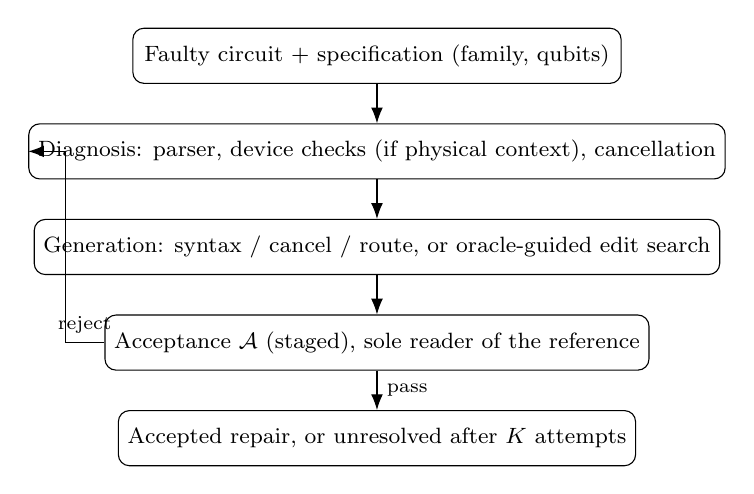
\begin{tikzpicture}[
  node distance=5mm,
  box/.style={draw, rounded corners, align=center, font=\footnotesize,
              minimum width=62mm, minimum height=7mm},
  arr/.style={-{Latex[length=2mm]}}]
\node[box] (in) {Faulty circuit + specification (family, qubits)};
\node[box, below=of in] (diag) {Diagnosis: parser, device checks (if physical context), cancellation};
\node[box, below=of diag] (gen) {Generation: syntax / cancel / route, or oracle-guided edit search};
\node[box, below=of gen] (val) {Acceptance $\mathcal{A}$ (staged), sole reader of the reference};
\node[box, below=of val] (out) {Accepted repair, or unresolved after $K$ attempts};
\draw[arr] (in) -- (diag);
\draw[arr] (diag) -- (gen);
\draw[arr] (gen) -- (val);
\draw[arr] (val) -- node[right, font=\scriptsize] {pass} (out);
\draw[arr] (val.west) -- ++(-5mm,0)
  node[midway, above, font=\scriptsize, sloped] {reject}
  |- (diag.west);
\end{tikzpicture}
\caption{Bounded repair loop. The reference reaches only the acceptance
predicate and, wrapped as a query-counted oracle, the generation stage.
Diagnostic feedback carries the rejecting stage and, on a semantic rejection, a
counterexample test.}
\label{fig:arch}
\end{figure}

\subsection{Deterministic repairs}

Syntax faults are repaired by token-level recovery (keyword and semicolon
restoration, restoring a lost closing bracket after its index). Redundancy is
repaired by DAG inverse cancellation. A physical fault is repaired, when physical
context is on, by dropping idle delays beyond $150\,\mu\mathrm{s}$ and then
routing with swap-in/swap-back followed by cancellation. The router is the same
construction used to build physical-fault references; routing agreement is
therefore partly by construction (Section~\ref{sec:threats}).

\subsection{Oracle-guided edit search}

Structural and semantic faults are repaired by greedy hill climbing over
single-instruction edits, each costing one oracle query. The neighbourhood is
generic and not conditioned on a fault label:
\emph{analytic angle moves} (below); substitution of a parameter-free
single-qubit gate among $\{H,X,Y,Z,S,S^\dagger,T,T^\dagger\}$; rotation-axis
exchange; reversal of CX operands; re-targeting a single-qubit gate to another
qubit; deletion of an instruction; and insertion of $H$, $X$, adjacent CX or
adjacent SWAP at any position. Not in the neighbourhood, by design: two-qubit
gate substitution, insertion of rotations, and simultaneous multi-instruction
edits beyond the greedy depth of four steps.

\textbf{Analytic angle solving.} For a gate $e^{-i\theta G/2}$ with $G^2=I$
(single-qubit rotations) or a controlled phase $\mathrm{diag}(1,\dots,e^{i\theta})$,
the amplitude of any fixed input--output pair is $a e^{-i\theta/2}+be^{i\theta/2}$
or $a+be^{i\theta}$, so its squared modulus, and hence the suite score, is
\begin{equation}
f(\theta)=c_0+c_1\cos\theta+s_1\sin\theta .
\end{equation}
Three probes at $\theta\in\{0,2\pi/3,4\pi/3\}$ determine $(c_0,c_1,s_1)$ by a
well-conditioned $3\times3$ solve, and the maximiser is
$\theta^\star=\operatorname{atan2}(s_1,c_1)$ with predicted score
$c_0+\sqrt{c_1^2+s_1^2}$. A wrong angle is thus corrected in three queries per
rotation instruction, whatever the perturbation.

\textbf{Meet-in-the-middle scoring.} The score of every single-instruction edit
of a base circuit is computed from cached forward states (prefixes applied to the
suite inputs) and backward states (suffixes inverted and applied to the
reference outputs), so an edit costs one local gate application rather than a
full simulation. Values equal naive scoring to $10^{-10}$ (unit-tested); budget
accounting still charges one query per edit, and only scalars leave the oracle.

\textbf{Tabu diversification.} Submitted circuits enter a tabu set, so a retry
returns a different candidate and attempts are not spent on byte-identical
resubmissions.

\subsection{Counterexample-guided feedback}

When $\mathcal{A}$ rejects a candidate at the semantic stage and diagnostic
feedback is on, the oracle moves the pool state on which the candidate disagrees
most into the suite and the search restarts from the candidate with the enlarged
suite. This is counterexample-guided repair~\cite{solarlezama2006sketching}. It
makes the feedback ablation testable without a language model, because the
feedback now changes what the generator can know.

\section{Experimental Design}
\label{sec:design}

\textbf{Arms.} Table~\ref{tab:arms} lists the systems (Qiskit is also run at levels 0, 2 and 3). All run through the
same loop with the same $K=3$ and the same acceptance predicate. No system is
given the reference or the fault label.

\begin{table}[t]
\centering
\caption{Systems. P/U: physical context on/off; D/R: diagnostic feedback or bare
rejection.}
\label{tab:arms}
\footnotesize
\begin{tabular}{llccc}
\toprule
Code & Description & Phys. & Feedback & Oracle \\
\midrule
P+D & full agent & on & diag. & yes \\
P+R & bare rejection & on & bare & yes \\
U+D & no physical context & off & diag. & yes \\
U+R & no phys., bare rej. & off & bare & yes \\
Static & static repairs only & on & -- & no \\
PyZX & ZX simplification & -- & -- & no \\
P+D/Q & P+D, Qiskit router & on & diag. & yes \\
Qiskit & compiler only, O0--O3 & -- & -- & no \\
\bottomrule
\end{tabular}
\end{table}

\textbf{Experiments.} E1 (main): suite of 4 states, budget 8000 queries, the six
core arms plus the compiler and router arms (run afterwards on the same
circuits), all 1000 circuits. E2 (weak oracle): suite of 1 state ($\lvert 0\ldots0
\rangle$), same budget, the four factorial arms. E3 (budget sweep): suite of 4,
budgets $50,\dots,3200$, arms P+D and U+R.

\textbf{Statistics.} Pass@$k$ is the fraction accepted within $k$ attempts, read
from the attempt trace. Rates carry Wilson 95\% intervals. Outcomes are paired
binary variables, so contrasts use McNemar's exact test~\cite{mcnemar1947} on
discordant pairs with the paired risk difference and a Newcombe method-10
interval~\cite{newcombe1998paired}; Holm correction~\cite{holm1979} is applied
over the rows of each contrast table. Six contrasts were fixed before
running; the compiler and router contrasts were added after the first results
and are labelled as such here. Resource overhead is gate count relative to the reference over accepted
repairs only. All runs are deterministic.

\section{Results}
\label{sec:results}

\subsection{E1: main configuration}

Table~\ref{tab:rates} and Fig.~\ref{fig:passk} give the primary outcomes. P+D is
accepted on $97.0\%$ of circuits within three attempts (95\% CI $[95.7,97.9]$) and
every final candidate is physically valid. Without physical context the rate is
$77.0\%$ $([74.3,79.5])$ and $80.1\%$ of final candidates are valid. Static repair
without an oracle reaches $60.0\%$ and ZX simplification $5.0\%$. Accepted
repairs of the oracle arms are within $0.2\%$ of the reference in gate count on
average; PyZX output is $156.8\%$ larger.

\begin{table*}[t]
\centering
\caption{Acceptance under the shared predicate, $n=1000$ circuits, attempt budget $K=3$. CI: Wilson 95\%. P/U = physics context on/off; D/R = diagnostic feedback / bare rejection; Static = no oracle.}
\label{tab:rates}
\footnotesize
\setlength{\tabcolsep}{3pt}
\begin{tabular}{lrrrrrr}
\toprule
System & P@1 (\%) & P@3 (\%) & P@3 95\% CI & Phys.\ valid (\%) & Attempts & Queries \\
\midrule
P+D & 97.0 & 97.0 & [95.7, 97.9] & 100.0 & 1.06 & 553 \\
P+R & 97.0 & 97.0 & [95.7, 97.9] & 100.0 & 1.06 & 555 \\
U+D & 77.0 & 77.0 & [74.3, 79.5] & 80.1 & 1.46 & 963 \\
U+R & 77.0 & 77.0 & [74.3, 79.5] & 80.1 & 1.46 & 965 \\
Static & 60.0 & 60.0 & [56.9, 63.0] & 100.0 & 1.80 & 0 \\
PyZX & 5.0 & 5.0 & [3.8, 6.5] & 15.1 & 2.90 & 0 \\
\bottomrule
\end{tabular}
\end{table*}


\begin{figure}[t]
\centering
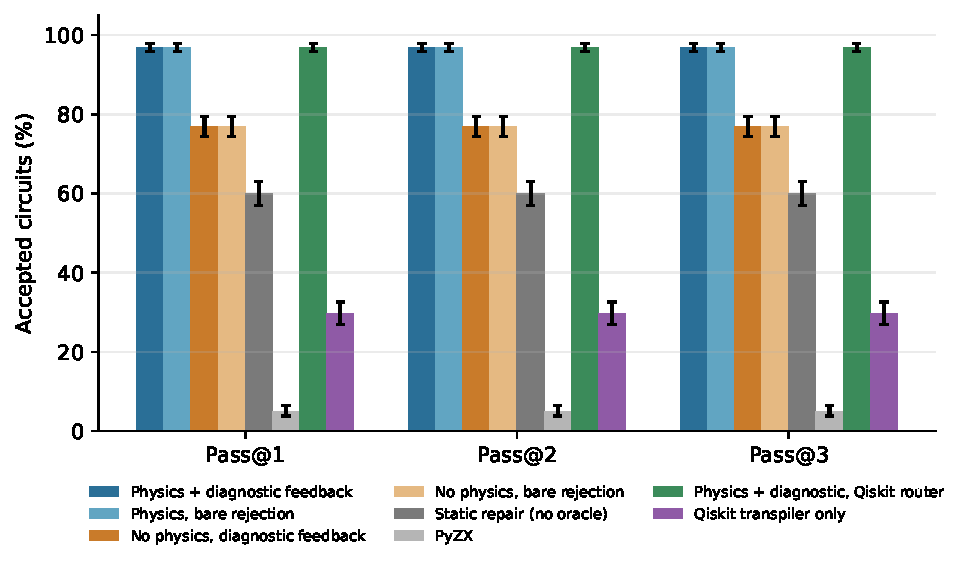
\includegraphics[width=\columnwidth]{pass_at_k.pdf}
\caption{Pass@$k$ in E1 with Wilson 95\% intervals. Attempts beyond the first
add nothing in this regime.}
\label{fig:passk}
\end{figure}

Table~\ref{tab:contrasts} gives the contrasts. The physical-knowledge effect is
$+0.200$ ($[0.176,0.226]$; 200 circuits repaired by the physical arm and none in
the reverse direction) and is the same with feedback on and off. The oracle
effect is $+0.370$ ($[0.340,0.400]$). Diagnostic feedback has no effect: 0
discordant pairs in both comparisons.

\begin{table*}[t]
\centering
\caption{Pre-specified paired contrasts (exact McNemar; Newcombe interval on the paired risk difference; Holm correction over the 18 rows shown).}
\label{tab:contrasts}
\footnotesize
\setlength{\tabcolsep}{3pt}
\begin{tabular}{lrrrrr}
\toprule
contrast & metric & b10 & b01 & RD [95\% CI] & p\_holm \\
\midrule
physics context (feedback on) & Pass@1 & 200 & 0 & +0.200 [+0.176, +0.226] & $1.5\times 10^{-59}$ \\
physics context (feedback on) & Pass@3 & 200 & 0 & +0.200 [+0.176, +0.226] & $1.5\times 10^{-59}$ \\
physics context (feedback off) & Pass@1 & 200 & 0 & +0.200 [+0.176, +0.226] & $1.5\times 10^{-59}$ \\
physics context (feedback off) & Pass@3 & 200 & 0 & +0.200 [+0.176, +0.226] & $1.5\times 10^{-59}$ \\
diagnostic feedback (physics on) & Pass@1 & 0 & 0 & +0.000 [-0.004, +0.004] & 1 \\
diagnostic feedback (physics on) & Pass@3 & 0 & 0 & +0.000 [-0.004, +0.004] & 1 \\
diagnostic feedback (physics off) & Pass@1 & 0 & 0 & +0.000 [-0.002, +0.002] & 1 \\
diagnostic feedback (physics off) & Pass@3 & 0 & 0 & +0.000 [-0.002, +0.002] & 1 \\
behavioural oracle & Pass@1 & 370 & 0 & +0.370 [+0.340, +0.400] & $1.2\times 10^{-110}$ \\
behavioural oracle & Pass@3 & 370 & 0 & +0.370 [+0.340, +0.400] & $1.2\times 10^{-110}$ \\
transformation baseline & Pass@1 & 920 & 0 & +0.920 [+0.901, +0.935] & $4.1\times 10^{-276}$ \\
transformation baseline & Pass@3 & 920 & 0 & +0.920 [+0.901, +0.935] & $4.1\times 10^{-276}$ \\
compiler baseline & Pass@1 & 673 & 0 & +0.673 [+0.643, +0.701] & $8.2\times 10^{-202}$ \\
compiler baseline & Pass@3 & 673 & 0 & +0.673 [+0.643, +0.701] & $8.2\times 10^{-202}$ \\
extended edit neighbourhood (added after E1) & Pass@1 & 18 & 2 & +0.016 [+0.008, +0.026] & 0.00282 \\
extended edit neighbourhood (added after E1) & Pass@3 & 20 & 2 & +0.018 [+0.009, +0.029] & $9.7\times 10^{-4}$ \\
router choice (own vs Qiskit) & Pass@1 & 0 & 0 & +0.000 [-0.004, +0.004] & 1 \\
router choice (own vs Qiskit) & Pass@3 & 0 & 0 & +0.000 [-0.004, +0.004] & 1 \\
\bottomrule
\end{tabular}
\end{table*}


\textbf{The physical-knowledge effect is a capability effect confined to the
physical class.} Table~\ref{tab:class} shows $100\%$ against $0\%$ on the 200
physical-fault circuits and identical rates on the other four classes. An arm
without delay trimming and routing cannot repair a routing or coherence fault, so
this contrast measures the availability of those operations, which we report
openly, rather than any improvement in semantic reasoning, on which the arms are
indistinguishable. In the unconstrained arms $199$ of the $200$ physical faults
are rejected at the connectivity ($96$) or coherence ($103$) stage
(Table~\ref{tab:stages}); one is rejected at the semantic stage.

\begin{table*}[t]
\centering
\caption{Pass@3 (\%) by injected fault class (200 circuits per class). P/U = physics context on/off; D/R = diagnostic feedback / bare rejection; Static = no oracle; P+D/E = P+D with the extended edit neighbourhood; P+D/Q = P+D with Qiskit routing; Qiskit On = transpiler only at optimisation level n.}
\label{tab:class}
\footnotesize
\setlength{\tabcolsep}{3pt}
\begin{tabular}{lrrrrrrrrrrrr}
\toprule
bug\_type & P+D & P+R & U+D & U+R & Static & PyZX & P+D/E & P+D/Q & Qiskit O1 & Qiskit O0 & Qiskit O2 & Qiskit O3 \\
\midrule
gate\_redundancy & 100.0 & 100.0 & 100.0 & 100.0 & 100.0 & 25.0 & 100.0 & 100.0 & 100.0 & 0.0 & 100.0 & 100.0 \\
physics\_violation & 100.0 & 100.0 & 0.0 & 0.0 & 100.0 & 0.0 & 100.0 & 100.0 & 48.5 & 48.5 & 48.5 & 48.5 \\
semantic\_deviation & 100.0 & 100.0 & 100.0 & 100.0 & 0.0 & 0.0 & 99.0 & 100.0 & 0.0 & 0.0 & 0.0 & 0.0 \\
structural & 85.0 & 85.0 & 85.0 & 85.0 & 0.0 & 0.0 & 95.0 & 85.0 & 0.0 & 0.0 & 0.0 & 0.0 \\
syntax & 100.0 & 100.0 & 100.0 & 100.0 & 100.0 & 0.0 & 100.0 & 100.0 & 0.0 & 0.0 & 0.0 & 0.0 \\
\bottomrule
\end{tabular}
\end{table*}


\begin{table*}[t]
\centering
\caption{Rejecting stage of the final attempt among unresolved circuits. P/U = physics context on/off; D/R = diagnostic feedback / bare rejection; Static = no oracle; P+D/Q = P+D with Qiskit routing; Qiskit = transpiler only.}
\label{tab:stages}
\footnotesize
\setlength{\tabcolsep}{3pt}
\begin{tabular}{lrrrrrrrr}
\toprule
final\_failed\_stage & P+D & P+R & U+D & U+R & Static & PyZX & P+D/Q & Qiskit \\
\midrule
coherence & 0 & 0 & 103 & 103 & 0 & 0 & 0 & 103 \\
connectivity & 0 & 0 & 96 & 96 & 0 & 264 & 0 & 0 \\
generation & 0 & 0 & 0 & 0 & 0 & 585 & 0 & 200 \\
minimality & 0 & 0 & 0 & 0 & 0 & 25 & 0 & 0 \\
semantic & 30 & 30 & 31 & 31 & 400 & 76 & 30 & 400 \\
\bottomrule
\end{tabular}
\end{table*}


\subsection{Fault modes and the limits of the neighbourhood}

Table~\ref{tab:mode} reports Pass@3 per fault mode. All semantic modes,
including the extended ones (scale, $\pi/3$ shift, compound), reach $100\%$:
angle solving corrects any single wrong angle, and the greedy path resolves two
simultaneous faults. The unresolved circuits (30, all in the structural class)
are concentrated where the neighbourhood is incomplete. Of the 11 circuits whose
removed instruction was a rotation or controlled phase, none is repaired,
because rotations are not insertable; removal of a CX, $H$ or $X$ is repaired in
all 42 cases and of a SWAP in $90\%$ of 21. Re-targeting a single-qubit gate is
repaired in $97\%$ of cases for $H$ but only $50\%$ for $R_z$ (12 circuits).
CX$\to$CZ replacement, absent from the neighbourhood, is repaired in $63\%$ of
27 circuits (GHZ $89\%$, QAOA $56\%$, VQE $44\%$), which requires a two-edit
path. These cells, not the aggregate, indicate what the agent cannot do.

\begin{table*}[t]
\centering
\caption{Pass@3 (\%) by fault mode. ``legacy'' modes come from the v1 injector; ``extended'' modes were added in v2. P/U = physics context on/off; D/R = diagnostic feedback / bare rejection; Static = no oracle.}
\label{tab:mode}
\footnotesize
\setlength{\tabcolsep}{3pt}
\begin{tabular}{lrrrrr}
\toprule
bug\_type & fault\_mode & mode\_family & P+D & U+R & n \\
\midrule
gate\_redundancy & cxcx & legacy & 100.0 & 100.0 & 64 \\
gate\_redundancy & hh & legacy & 100.0 & 100.0 & 61 \\
gate\_redundancy & xx & legacy & 100.0 & 100.0 & 75 \\
physics\_violation & coherence\_delay & legacy & 100.0 & 0.0 & 103 \\
physics\_violation & unmapped & legacy & 100.0 & 0.0 & 97 \\
semantic\_deviation & axis\_change & legacy & 100.0 & 100.0 & 14 \\
semantic\_deviation & compound & extended & 100.0 & 100.0 & 33 \\
semantic\_deviation & gate\_replace & legacy & 100.0 & 100.0 & 50 \\
semantic\_deviation & negate & legacy & 100.0 & 100.0 & 27 \\
semantic\_deviation & scale & extended & 100.0 & 100.0 & 16 \\
semantic\_deviation & shift\_pi2 & legacy & 100.0 & 100.0 & 30 \\
semantic\_deviation & shift\_pi3 & extended & 100.0 & 100.0 & 30 \\
structural & invert\_cnot & legacy & 100.0 & 100.0 & 44 \\
structural & remove\_gate & legacy & 82.4 & 82.4 & 74 \\
structural & twoqubit\_replace & extended & 63.0 & 63.0 & 27 \\
structural & wrong\_qubit & legacy & 87.3 & 87.3 & 55 \\
syntax & corrupt\_keyword & legacy & 100.0 & 100.0 & 60 \\
syntax & illegal\_bracket & legacy & 100.0 & 100.0 & 50 \\
syntax & invalid\_gate & legacy & 100.0 & 100.0 & 37 \\
syntax & missing\_semicolon & legacy & 100.0 & 100.0 & 53 \\
\bottomrule
\end{tabular}
\end{table*}


\subsection{Compiler baseline and router robustness}

A standard compiler is the natural baseline for the physical class. The
\emph{Qiskit} arm runs the transpiler (trivial layout, SABRE routing onto the
device line, level-1 optimisation) and appends an exact permutation that undoes
the final layout, so its output implements the same unitary as its input and is
scored by the same predicate; it contains no repair logic. It is accepted on
$29.7\%$ of circuits ($[26.9,32.6]$): $100\%$ of redundancy faults (level-1
cancellation), $48.5\%$ of physical faults (all 97 unmapped circuits, none of the
103 over-long delays, which the transpiler leaves in place), and none of the
syntax, structural or semantic faults. P+D exceeds it by $+0.673$
($[0.643,0.701]$; 673 discordant circuits, none reversed), so compilation alone
covers less than a third of the benchmark even in its home class. Replacing the
agent's router by Qiskit's (P+D/Q) leaves acceptance unchanged (zero discordant
circuits). Across Qiskit optimisation levels the compiler-only rate is $9.7\%$
at level 0 (routing only: the 97 unmapped circuits), $29.7\%$ at level 1 and
likewise at levels 2 and 3, which add inverse cancellation; higher optimisation
does not erase the benchmark's faults, because none except redundancy can be
removed by compilation.

\subsection{E2: weak oracle}

With a suite of one state the first-attempt rate falls from $97.0\%$ to $86.9\%$
and feedback becomes decisive (Table~\ref{tab:weak}). P+D rises to $96.8\%$ at the
second attempt and $97.0\%$ at the third; P+R reaches only $88.1\%$
$([85.9,90.0])$. The feedback effect is $+0.089$ ($[0.072,0.108]$; 90 circuits
repaired with feedback and 1 without; Holm $p=3.0\times10^{-25}$) and is
identical with physical context on and off (Table~\ref{tab:weakc}). It is
concentrated in the semantic class ($98.5\%$ against $70.5\%$) and the structural
class ($86.5\%$ against $70.0\%$). A single state cannot distinguish a circuit
that lacks a rotation from one that has it; a counterexample supplies the
distinguishing input.

\begin{table*}[t]
\centering
\caption{Weak-oracle regime (initial suite = $|0\ldots0\rangle$ only; oracle budget unchanged). P/U = physics context on/off; D/R = diagnostic feedback / bare rejection; Static = no oracle; P+D/E = P+D with the extended edit neighbourhood; P+D/Q = P+D with Qiskit routing; Qiskit On = transpiler only at optimisation level n.}
\label{tab:weak}
\footnotesize
\setlength{\tabcolsep}{3pt}
\begin{tabular}{lrrrrrr}
\toprule
System & P@1 (\%) & P@3 (\%) & P@3 95\% CI & Phys.\ valid (\%) & Attempts & Queries \\
\midrule
P+D & 86.9 & 97.0 & [95.7, 97.9] & 100.0 & 1.16 & 584 \\
P+R & 86.9 & 88.1 & [85.9, 90.0] & 100.0 & 1.25 & 540 \\
U+D & 66.9 & 77.0 & [74.3, 79.5] & 80.0 & 1.56 & 910 \\
U+R & 66.9 & 68.1 & [65.1, 70.9] & 80.0 & 1.65 & 866 \\
\bottomrule
\end{tabular}
\end{table*}


\begin{table*}[t]
\centering
\caption{Paired contrasts in the weak-oracle regime (Holm over the 8 rows shown).}
\label{tab:weakc}
\footnotesize
\setlength{\tabcolsep}{3pt}
\begin{tabular}{lrrrrr}
\toprule
contrast & metric & b10 & b01 & RD [95\% CI] & p\_holm \\
\midrule
physics context (feedback on) & Pass@1 & 200 & 0 & +0.200 [+0.175, +0.225] & $1.0\times 10^{-59}$ \\
physics context (feedback on) & Pass@3 & 200 & 0 & +0.200 [+0.176, +0.226] & $1.0\times 10^{-59}$ \\
physics context (feedback off) & Pass@1 & 200 & 0 & +0.200 [+0.175, +0.225] & $1.0\times 10^{-59}$ \\
physics context (feedback off) & Pass@3 & 200 & 0 & +0.200 [+0.175, +0.225] & $1.0\times 10^{-59}$ \\
diagnostic feedback (physics on) & Pass@1 & 0 & 0 & +0.000 [-0.003, +0.003] & 1 \\
diagnostic feedback (physics on) & Pass@3 & 90 & 1 & +0.089 [+0.072, +0.108] & $3.0\times 10^{-25}$ \\
diagnostic feedback (physics off) & Pass@1 & 0 & 0 & +0.000 [-0.001, +0.001] & 1 \\
diagnostic feedback (physics off) & Pass@3 & 90 & 1 & +0.089 [+0.071, +0.107] & $3.0\times 10^{-25}$ \\
\bottomrule
\end{tabular}
\end{table*}


\subsection{E3: query budget}

Table~\ref{tab:budget} and Fig.~\ref{fig:budget} vary the per-repair oracle
budget with a suite of four states. Pass@3 of P+D rises from $77.7\%$ at 50
queries to $85.1\%$ (100), $88.3\%$ (200), $91.4\%$ (400), $93.7\%$ (800),
$95.6\%$ (1600), $96.7\%$ (3200) and $97.0\%$ at the default 8000, with
diminishing returns: $+7.4$ points from 50 to 100 queries, $+1.1$ from 1600 to
3200 and $+0.3$ from 3200 to 8000. The 600 syntax, redundancy and physical-fault
circuits that static repair resolves need no oracle and are accepted at any
budget, so the budget governs only the 400 structural and semantic circuits:
$44\%$ of them are repaired within 50 queries, $92\%$ within 3200. U+R trails
P+D by exactly $20.0$ points at every budget, the share of physical faults;
budget and physical context do not interact.

\begin{table}[t]
\centering
\caption{Pass@3 (\%) as a function of the per-repair oracle query budget (suite size 4). P/U = physics context on/off; D/R = diagnostic feedback / bare rejection; Static = no oracle; P+D/E = P+D with the extended edit neighbourhood; P+D/Q = P+D with Qiskit routing; Qiskit On = transpiler only at optimisation level n.}
\label{tab:budget}
\footnotesize
\setlength{\tabcolsep}{3pt}
\begin{tabular}{lrr}
\toprule
budget & P+D & U+R \\
\midrule
50 & 77.7 & 57.7 \\
100 & 85.1 & 65.1 \\
200 & 88.3 & 68.3 \\
400 & 91.4 & 71.4 \\
800 & 93.7 & 73.7 \\
1600 & 95.6 & 75.6 \\
3200 & 96.7 & 76.7 \\
\bottomrule
\end{tabular}
\end{table}


\begin{figure}[t]
\centering
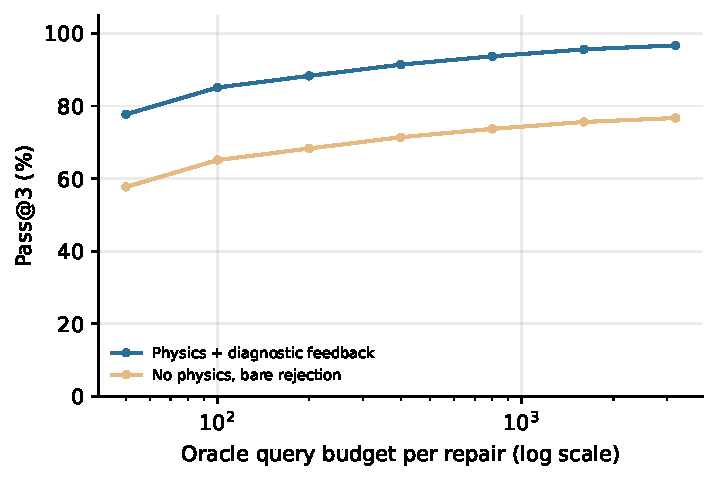
\includegraphics[width=0.9\columnwidth]{budget_curve.pdf}
\caption{Pass@3 as a function of the per-repair oracle query budget (E3).}
\label{fig:budget}
\end{figure}

\subsection{Oracle cost and overfitting}

Table~\ref{tab:cost} reports cost. The median searched repair in P+D uses
508 queries, the 95th percentile 2347, and counterexamples are rare (0.066 per
run). Accepted repairs cannot exhibit a suite--process gap above $0.01$ by
construction, so the gap is informative only among unresolved circuits: for 23
of the 30 unresolved final candidates of P+D, suite agreement exceeds exact
process fidelity by more than $0.01$, i.e.\ the candidate fits the test suite
better than it fits the specification.

\begin{table*}[t]
\centering
\caption{Oracle cost and overfitting of the search signal (searches that used the oracle). Gap = suite agreement minus exact process fidelity of the final candidate.}
\label{tab:cost}
\footnotesize
\setlength{\tabcolsep}{3pt}
\begin{tabular}{lrrrrr}
\toprule
System & Mean queries & p95 queries & Counterex. & Gap$>$0.01 (\%) & Time (s) \\
\midrule
P+D & 553 & 2347 & 0.07 & 2.3 & 0.5 \\
P+R & 555 & 2614 & 0.00 & 2.8 & 0.45 \\
U+D & 963 & 4601 & 0.07 & 4.5 & 0.57 \\
U+R & 965 & 4601 & 0.00 & 5.0 & 0.57 \\
\bottomrule
\end{tabular}
\end{table*}


\section{Threats to Validity and Limitations}
\label{sec:threats}

\textbf{Edit-inversion benchmark.} Faults are single- or double-instruction
edits and the neighbourhood contains their inverses. The $97\%$ rate therefore
characterises the agent on this fault distribution and says little about
unrestricted faults. The informative evidence is the per-mode table, the
weak-oracle regime and the budget sweep.

\textbf{Language and fault coverage.} The acceptance predicate compares unitaries,
device admissibility and noisy output distributions, so it covers the purely
unitary subset of OpenQASM~3~\cite{cross2022openqasm3}. Control flow, timing,
\texttt{measure}, \texttt{reset} and declared inputs and outputs need structural
or path-level oracles that we do not implement. Empirical studies of real
quantum bugs report that a large share concern API usage, platform and
cross-layer behaviour rather than gate-level edits~\cite{luo2022bugfixes,
paltenghi2021bugs}, and some of these (measurement wiring, output format,
declaration errors) are not observable in the unitary at all. Our five classes
therefore do not represent field prevalence; a v3 benchmark should include
non-single-gate and non-unitary-observable faults (\texttt{docs/ROADMAP.md}).

\textbf{Routing by construction.} The agent's default router equals the
construction used to build physical-fault references. We tested this directly by
swapping in Qiskit's SABRE router with an exact final-layout undo: acceptance is
unchanged ($97.0\%$, zero discordant circuits), and the routed circuits are
$1.1\%$ smaller than the reference on average, so agreement is not an artefact
of sharing a router. The physical-knowledge contrast remains a capability
contrast (Section~\ref{sec:results}).

\textbf{Oracle strength.} Agreement on a handful of input states is a weaker
specification than a full test suite, and the oracle returns scores of many
candidate edits, which is substantial information about the reference. We bound
this by counting every edit as a query and by measuring the overfitting gap;
the budget and suite size are experimental variables, not hidden constants.

\textbf{Physical model.} Connectivity is checked on virtual indices under the
identity layout; the noise model is depolarising with analytic readout error;
FakeSherbrooke is a model, not a live device with calibration drift. A
routing-aware or transpiled evaluation would be strictly more demanding; initial
placement, routing and calibration-aware mapping change success rates
substantially on superconducting hardware~\cite{murali2019noise,nation2025benchmark},
so identity-layout validity is a necessary rather than sufficient condition.
Exact unitary comparison does not scale: the validator therefore also offers a
sampled average-fidelity check (and skips the density-matrix noise stage) above
ten qubits, which gives one-sided statistical evidence only, and
structure-aware verification such as automata-based~\cite{chen2023automata} or
ZX-based~\cite{peham2022zx} equivalence checking would be the principled
replacement. All reported results use the exact check ($\le 8$ qubits).

\textbf{Missing baselines.} No language model was executed, because no API key
was configured; the repository contains the language-model path but every
reported number is from the deterministic path, so nothing here is evidence
about language-model repair. We report no externally executed QBugLM run.

\textbf{Statistics.} The 1000 circuits are not independent draws of real
faults; they are a generated population, so intervals describe sampling over
that population. Three circuit families and a fixed fault taxonomy limit
generalisation.

\section{Conclusion}

Reported success rates for quantum-circuit repair depend on conditions that are
easy to violate silently: an information boundary around the reference, a
benchmark whose references satisfy the predicate, and faults the predicate can
detect. An audit found all three broken in an existing physics-constrained
repair benchmark, and a corrected protocol and benchmark remove the defects
while making the remaining limitations measurable. On the corrected benchmark a
repair agent with analytic angle solving and oracle-guided search is accepted on
$97.0\%$ of circuits at a matched budget of three attempts; the contribution of
physical knowledge is confined to the physical fault class, oracle access is
what separates semantic repair from static repair, and diagnostic feedback
matters when the oracle is weak. The natural next steps are a language-model
configuration, harder fault distributions outside the edit neighbourhood, and
evaluation across device models and calibration snapshots.

\section*{Acknowledgment}

The author thanks the open-source quantum software community.

\bibliographystyle{IEEEtran}
\bibliography{references}

\end{document}
